\documentclass[../main.tex]{subfiles}
\graphicspath{{\subfix{../images/}}}

\begin{document}

\begin{enumerate}
    \item[a)] Performance Achieved on Ultra96 Mapped Design: The throughput of our application is calculated based on the compression latency. The throughput calculation follows the following formula:
        
        $$
        ApplicationThroughput = \frac{\frac{BytesReadFromEthernet \times 8}{1000000}}{TotalCompressionLatency}
        $$
        
        \noindent In determining the compression latency, we utilized the stopwatch class by encapsulating the start and stop calls around our top function. This top function encompasses all the sub stages, such as CDC, SHA, DEDUP, LZW and includes writing data to the compressed file.  \\
        
        \noindent \textbf{Application Throughput: Linux.tar (Size: 200273920 B)(Binary File)} \\
        The throughput achieved is \textbf{71.237 Mb/s}. The intermediate throughputs were 1211.76 Mb/s for CDC, 728.032 Mb/s for SHA, 7593.07 Mb/s for Dedup, and 95.3945 Mb/s for LZW. Our output file is compressed to 95829565 Bytes. These values were determined from the “Linux.tar” test case. \\
        
        \noindent \textbf{Application Throughput: Franklin.txt (Size: 399054 B)(Text File)} \\
        Throughput achieved is \textbf{67.443 Mb/s}. The intermediate throughputs were 1178.01 Mb/s for CDC, 713.09 Mb/s for SHA, 8704.41 Mb/s for Dedup, and 92.6546 Mb/s for LZW. Our output file is compressed to 291731 Bytes. These values were determined from the “Franklin.txt” test case.  \\
        
        \newpage
        
        Terminal Output Linux Tar and Franklin respectively:
        \begin{figure}[H]
            \centering
            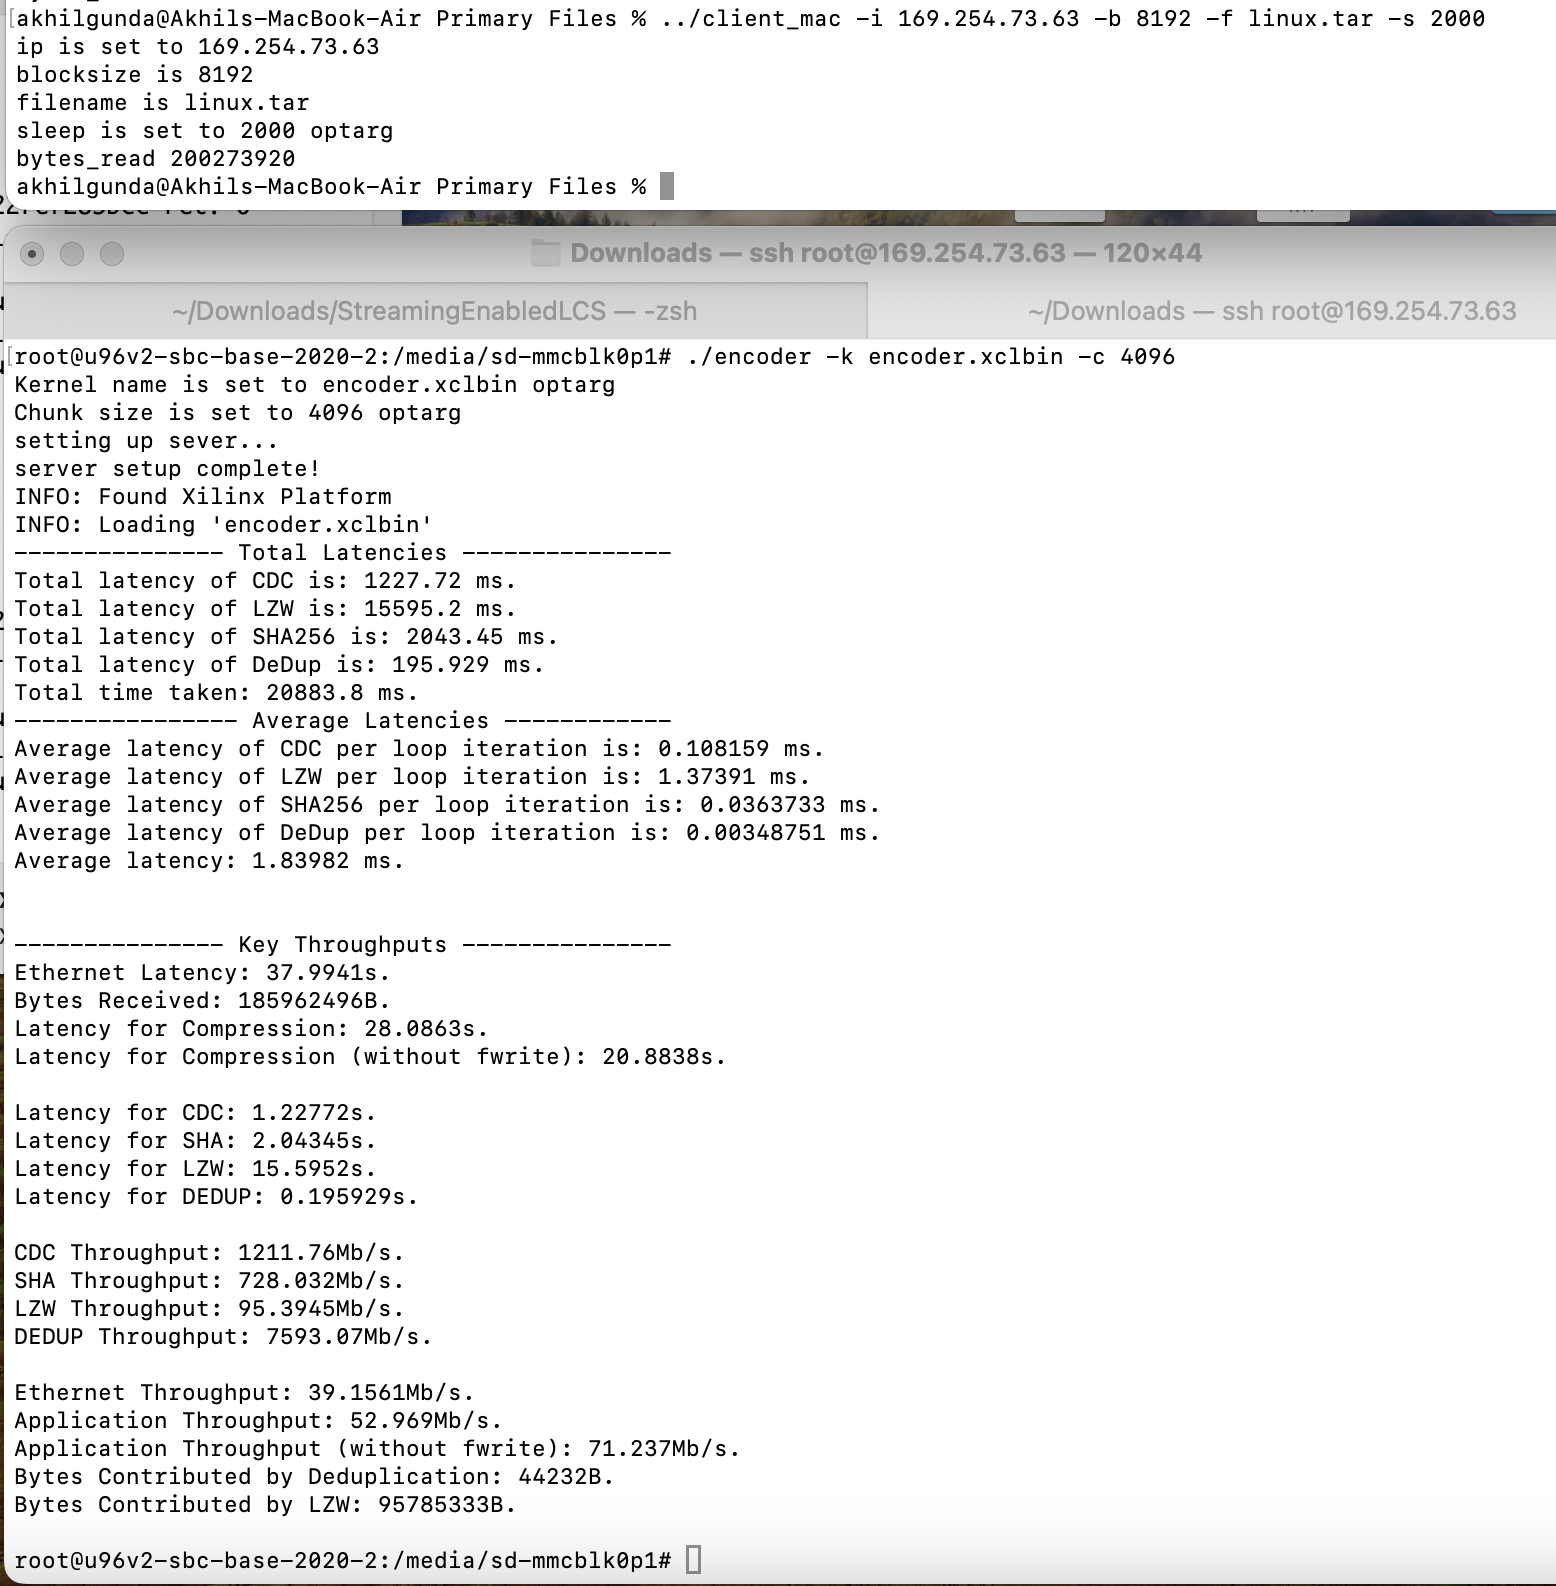
\includegraphics[width=0.63\linewidth]{Images/image9.png}
            \caption{Linux Tar}
            \label{fig:linux_tar}
        \end{figure}
        
        \begin{figure}[H]
            \centering
            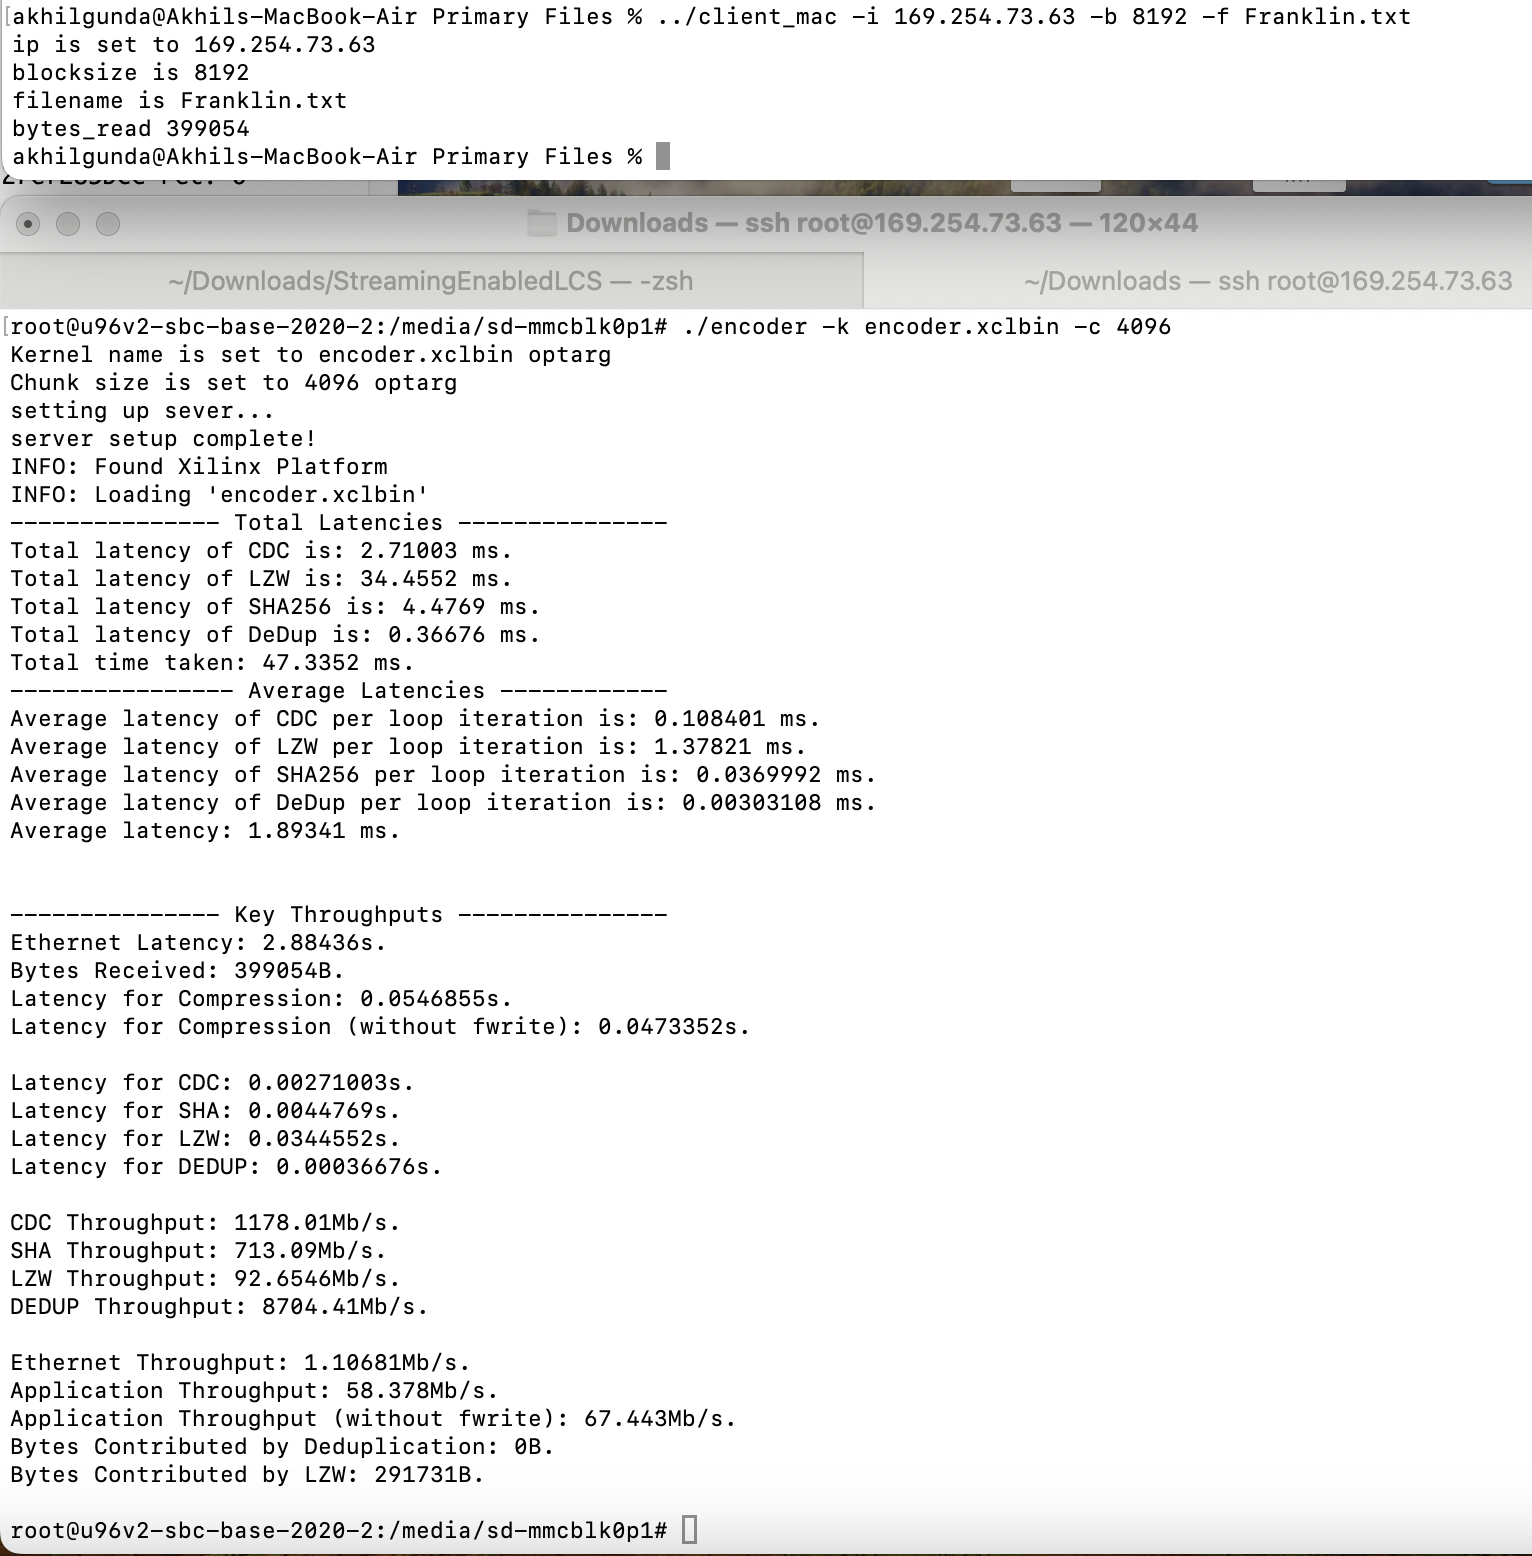
\includegraphics[width=0.63\linewidth]{Images/image22.png}
            \caption{Franklin Text File}
            \label{fig:franklin}
        \end{figure}
        
        Decode Diff Outputs for Linux.tar and Franklin.txt:
        \begin{figure}[H]
            \centering
            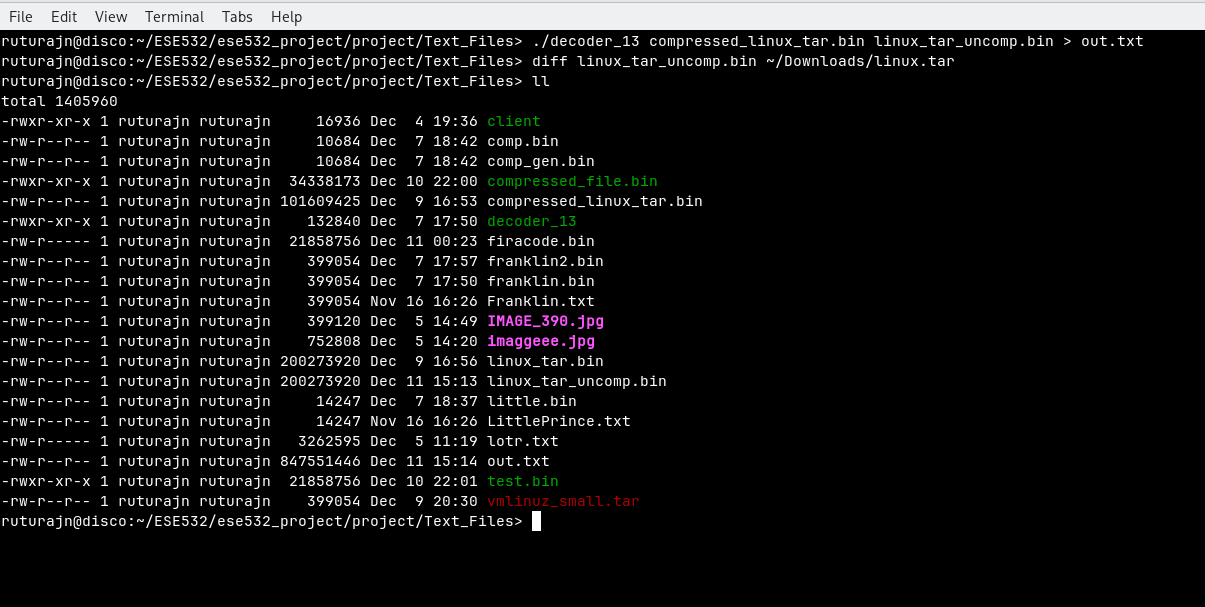
\includegraphics[width=0.63\linewidth]{Images/image27.png}
            \caption{Linux Tar Decoder Diff}
            \label{fig:linux_tar_diff}
        \end{figure}
        
        \begin{figure}[H]
            \centering
            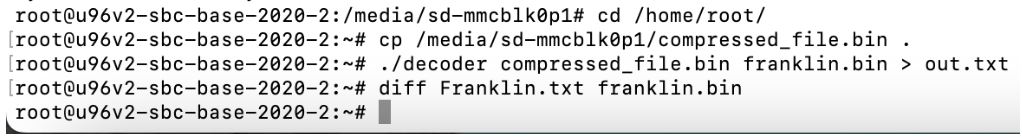
\includegraphics[width=0.7\linewidth]{Images/image28.png}
            \caption{Franklin Decoder Diff}
            \label{fig:franklin_diff}
        \end{figure}

    \vspace{1cm}

    \textbf{Vivado Analysis:}
    \begin{itemize}
        \item Power Consumption for this Design: The estimated total on-chip power is \textbf{2.803 W}.
        \begin{figure}[H]
            \centering
            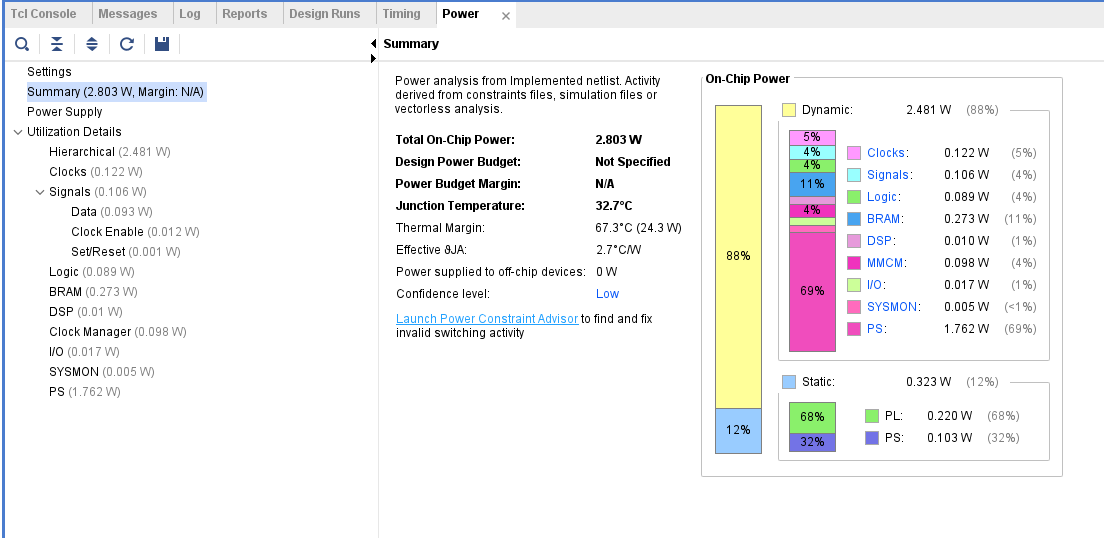
\includegraphics[width=0.7\linewidth]{Images/image25.png}
            \caption{Power Consumption}
            \label{fig:power_consp}
        \end{figure}

        \newpage

        \item Resource Utilization:
        \begin{figure}[H]
            \centering
            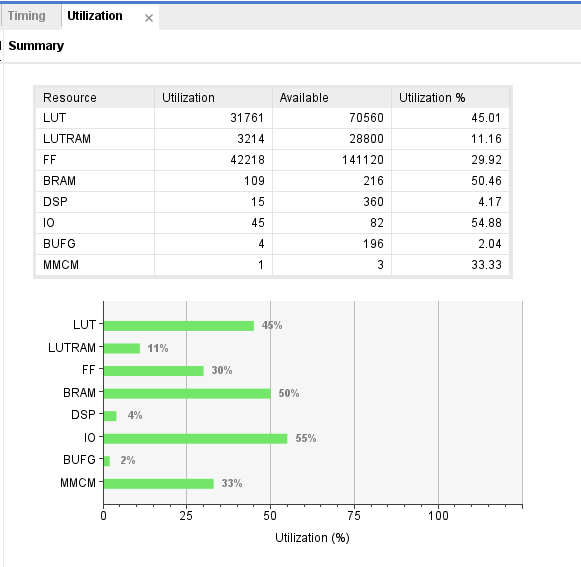
\includegraphics[width=0.65\linewidth]{Images/image10.png}
            \caption{Power Consumption}
            \label{fig:power_consp}
        \end{figure}
        
    \end{itemize}

    \vspace{1cm}

    \item[b)] Task Decomposition: For our final implementation, we receive data in buffers of 16KB from the client. Since we have moved to a block size of 8192, we are receiving 16KB in 2 packets. 

    Once we receive all of the 16KB data from the client, this is sent to the CDC function which makes multiple chunks of 4KB. We are using a different version of CDC called the Fast CDC which ensures that none of the chunks are greater than 4KB. This implementation of Fast CDC uses the GEAR hash. Chunks could be smaller than 4KB but we perform a hard chunk at 4KB. This version of Fast CDC performs a modulus in a different way as opposed to the regular CDC functionality. This works by skipping sub-minimum chunk cut-points. In this implementation, if the current chunking position is
    less that the average chunk size the modulus operation with the hash is performed with a value higher than the average chunk size and if the current chunking position is greater than the average chunk size the modulus operation with the hash is performed with a value smaller than
    the average chunk size. This ensures an even distribution of chunk sizes. This is how, a chunk is declared. If not, it declares a hard chunk of 4KB by looking at the previous chunk boundary. 
    
    Once all these chunks are made, SHA generates a 256 bit digest for each of these chunks. We have mapped the SHA computation onto the NEON registers which provided a substantial speedup over the software SHA implementation. This was implemented using the MPSOC library that was given in the project handout. This implementation uses the SHA cryptographic intrinsics as well as the NEON intrinsics. 
    
    These chunk fingerprints are used as keys in the hash table in the Deduplication stage. Fingerprints associated with duplicate chunks are only added to the hash table once. As of our current implementation, we are performing LZW on each of these chunks irrespective of it being a duplicate or not. This is because branch statements in our kernel were proving to slow down the overall application. Hence, we chose to perform LZW compression on every chunk regardless of it being a duplicate or not. Then on the basis of the output of the Deduplication stage, we decide whether to write just the header or the compressed codes in the form of packets to the file. 

    \begin{figure}[H]
        \centering
        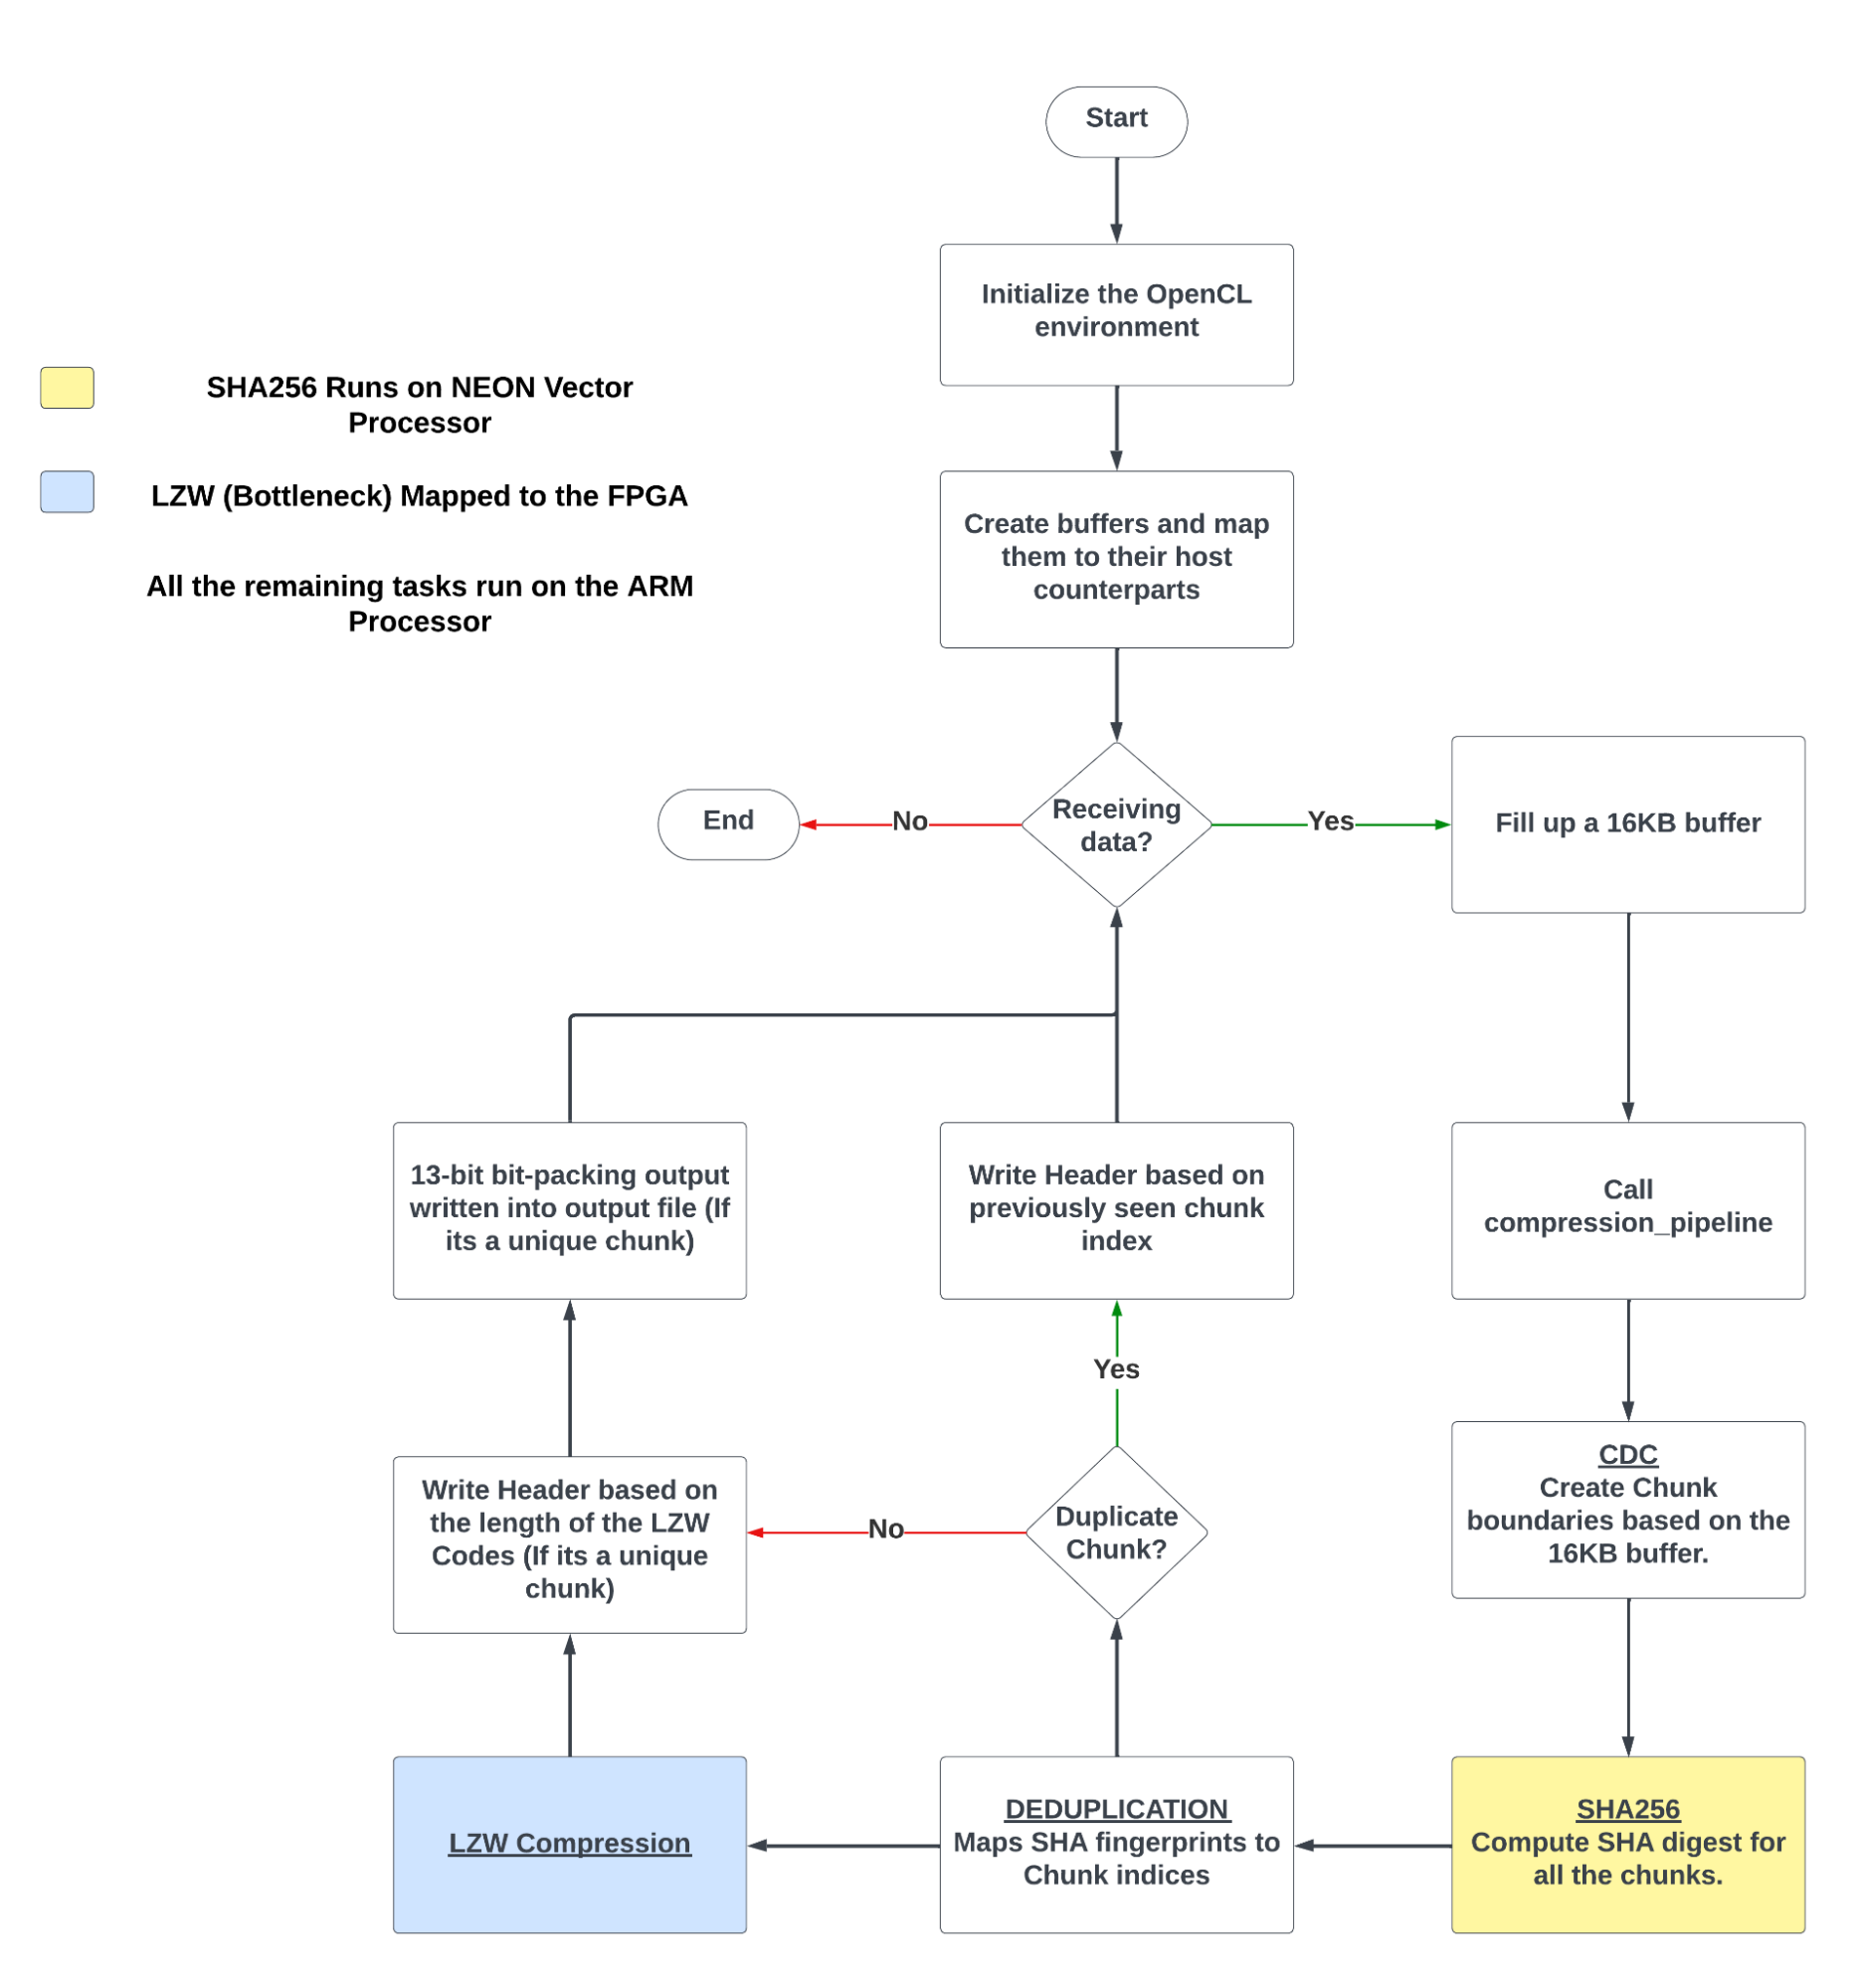
\includegraphics[width=0.85\linewidth]{../Images/image23.png}
        \caption{Flowchart}
        \label{fig:flowchart}
    \end{figure}

    \newpage

    \item[c)] Compression Achieved: \\
    \newline
    For the test case - Franklin.txt file, we achieved a compression ratio of,

    $$
    \frac{CompressedFileSize}{OriginalFileSize} = \frac{291731}{399054} = 0.73
    $$

    For the test case - Linux.tar file, we achieved a compression ratio of,

    $$
    \frac{CompressedFileSize}{OriginalFileSize} = \frac{95829565}{200273920} = 0.48
    $$

    \item[d)] Parallelism:
    \begin{enumerate}
        \item[1.]  For our CDC implementation, we tried to precalculate and store the power values in a local buffer. Since the hash calculation was using powers of 3 up to 17 repetitively for each iteration, we decided to hand calculate these and store them in an array from which they can be read for hash calculations. This made our CDC significantly quicker. To further optimize our CDC, we changed to FastCDC which used the GEAR hash and skips sub-minimum chunk cut-points. This made our final CDC implementation much faster as opposed to regular CDC. 

        CDC throughput before changing to FastCDC: 377.822 Mb/s \\
        CDC throughput after adapting the FastCDC implementation : 1185.7 Mb/s
        Speedup: 3.138x

        \item[2.] For the SHA implementation, we changed our software implementation of SHA 256 with the NEON intrinsics version of the implementation. This was implemented using the MPSOC library that was given in the project handout. This implementation uses the SHA cryptographic intrinsics as well as the NEON intrinsics which gives us significant speedup for the SHA since it uses 8 vector lanes. 

        SHA latency with the software implementation: 0.00058189 s \\
        SHA latency with the NEON intrinsics implementation: 0.00028 s \\
        Speedup: 2.078x

        \item[3.] Pipelining and parallelism can also be exploited within the kernel by enabling streams and data flow between the load, compute and store functions of the LZW compression. These streams act as a FIFO buffer from which data can be written to or read from each iteration. Functions within the dataflow region can execute concurrently. 

        We tried to use the dataflow pragma to enable data flow between the load, compute and store function to speed up the kernel. Although, we weren’t able to successfully complete it due to issues with synchronization in the output stream generated by the compute function. We noticed that with the dataflow pragma the C simulation worked perfectly fine, and the synthesis also passed, but the post C checking in co-simulation failed due to the output array being filled to zeros. 

        \item[4.] To exploit parallelism using threads in the host code, we tried to map the data collection from the ethernet on one thread and the compression\_pipeline function to another thread. This way we could use double buffering to fill data up in a buffer while another buffer is being processed on. Due to this our data processing pipeline is never waiting for data. Although this too didn’t work out, and we were facing issues with the two buffers that were setup, which resulted in a segmentation fault at the end of the application.
 
    \end{enumerate}

    \item[e)] Zynq Resource Mapping:
    
    \begin{table}[H]
        \centering
        \begin{tabular}{|c|c|c|c|} \hline 
             \textbf{Application}&  \textbf{Hardware}&  \textbf{Memory}& \textbf{FPGA Resource}\\
             \textbf{Stage}&  & \textbf{Utilization} & \textbf{Utilization}\\ \hline
             Encoder&  ARM Processor&  145KB& 0\\ \hline 
             CDC&  ARM Processor&  17KB& 0\\ \hline
             &  NEON Vector&  & \\
             SHA&  Processor +&  10KB& 0\\
             & ARM Processor&  & \\ \hline 
             DEDUP&  ARM Processor&  500 KB (Worst Case)& 0\\ \hline 
             &  &  Any memory used &LUTs: 48550 \\
             LZW&  FPGA&  in the host is  &FFs: 11269 \\
             &  &  included in the &DSPs: 3 \\
             &  &  Encoder &BRAM\_18Ks: 187 \\ \hline
        \end{tabular}
        \caption{Zynq Resource Mapping}
        \label{tab:zynq_mapping}
    \end{table}

    \begin{figure}[H]
        \centering
        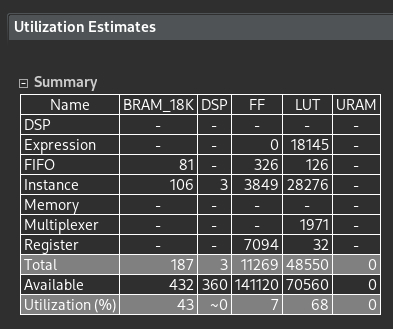
\includegraphics[width=0.5\linewidth]{Images/image15.png}
        \caption{Vitis Resource Utilization}
        \label{fig:vitis_util}
    \end{figure}

    \vspace{1cm}

    
    The following screenshot shows the breakdown of the resource utilization on the FPGA for our LZW kernel.

    \begin{figure}[H]
        \centering
        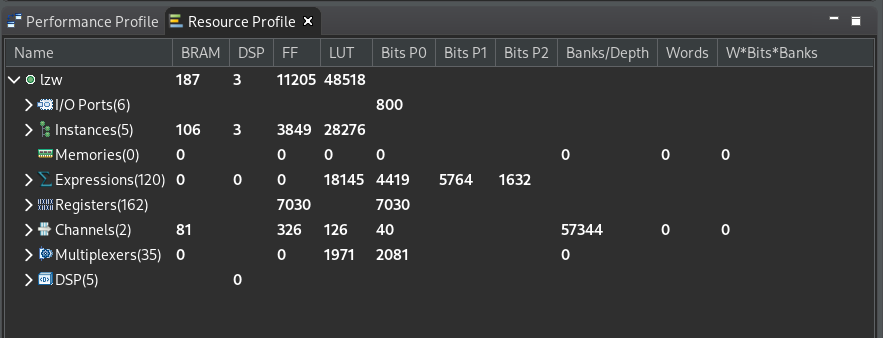
\includegraphics[width=0.7\linewidth]{Images/image17.png}
        \caption{Vitis Resource Profile}
        \label{fig:vitis_res_profile}
    \end{figure}

    \item[f)] Performance Model: \\
    Our final implementation consists of only 1 kernel/ compute unit. Hence, that will be our LZW throughput. The throughput is going to be defined by the bottleneck or the slowest operation. Since, LZW is our bottleneck, it is going to define our overall performance/ throughput to a large extent. Since everything is currently running on 1 thread, our overall application throughput is going to be min (CDC, SHA, Deduplication , LZW Compression). \\
    The overall application throughput does not match LZW’s throughput because our current implementation does not overlap the computation of LZW with that of the other functions. As a result of which, the overall application throughput is a little lesser than the throughput of LZW. \\

    
    \begin{table}[H]
        \centering
        \begin{tabular}{|c|c|} \hline 
             \textbf{Stage}& \textbf{Latency (ms)}\\ \hline 
             CDC& 2.71\\ \hline 
             SHA& 4.47\\ \hline 
             DEDUP& 0.36\\ \hline 
             LZW& 34.45\\ \hline
        \end{tabular}
        \caption{Latencies}
        \label{tab:latencies}
    \end{table}
    
    Total Latency: 41.99 ms \\
    
    Total Application Latency(including migrating memory back and forth from the host): 47.33 ms \\
    $$
    ModeledThroughput = \frac{SizeOfFranklin}{TotalLatency} = \frac{\frac{399054 \times 8}{1000000}}{47.33} = 67.45 Mb/s
    $$
    
    The reason this does not match our actual throughput is because of memory transfer overheads.


    \item[g)] Current Bottleneck Preventing Higher Performance: \\
    The bottleneck in our final implementation continues to be the LZW compression. To improve its performance, we moved the LZW onto the FPGA and tried a variety of methods to improve it. The screenshot below shows the Application timeline of our kernel in Vitis Analyzer.

    \begin{figure}[H]
        \centering
        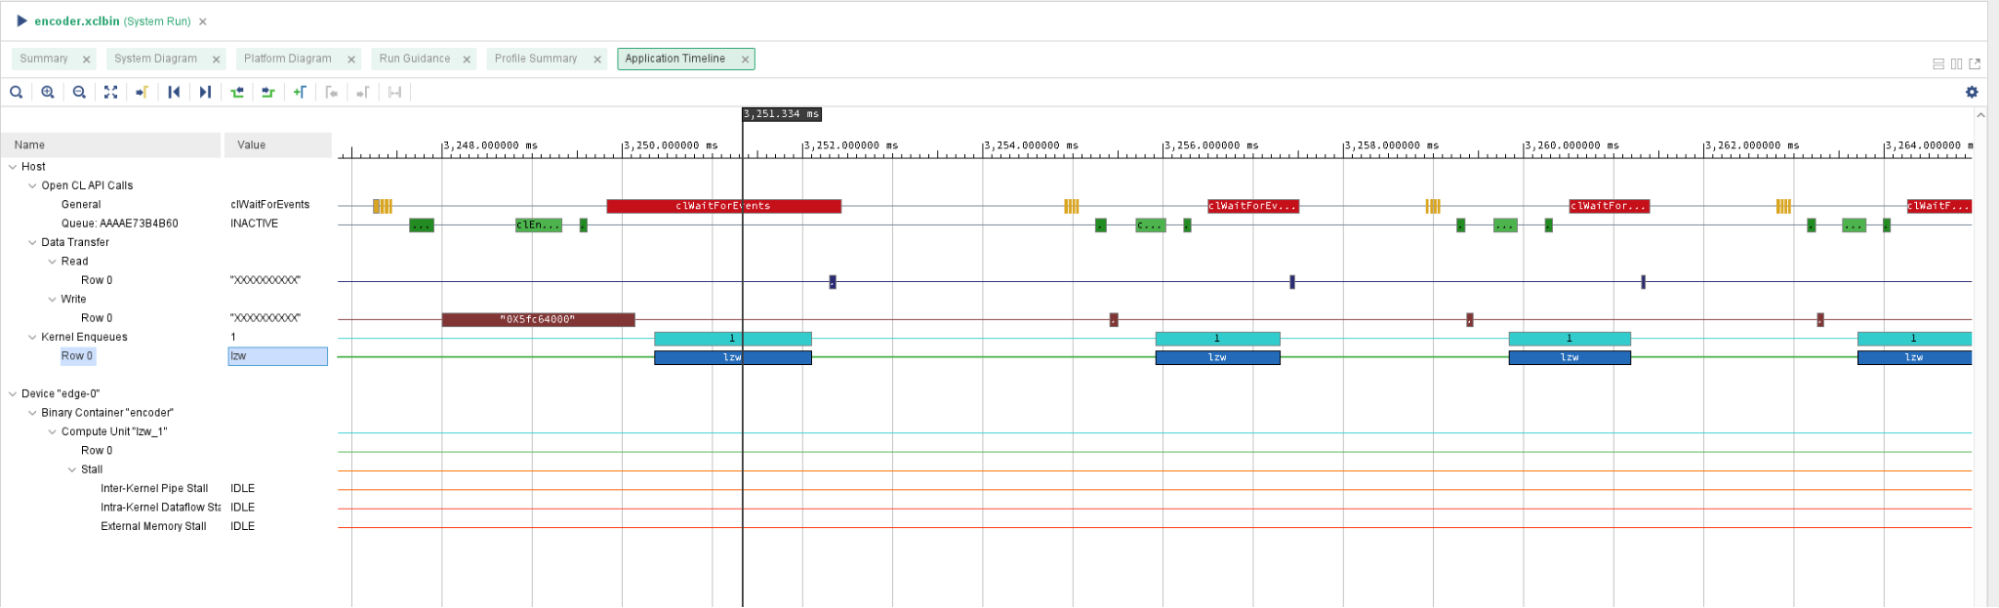
\includegraphics[width=0.8\linewidth]{Images/image13.png}
        \caption{Timeline Trace}
        \label{fig:timeline}
    \end{figure}
 
\end{enumerate}
\end{document}